\section{Slope of a Line}

In this section, you will learn to:
\begin{enumerate}
    \item Find the slope of a line.
    \item Graph the line if a point and the slope are given.
\end{enumerate}

In the last section, we learned to graph a line by choosing two points on the line. A graph of a line can also be determined if one point and the "steepness" of the line is known. The number that refers to the steepness or inclination of a line is called the slope of the line. From previous math courses, many of you remember slope as the "rise over run," or "the vertical change over the horizontal change" and have often seen it expressed as:
\[
\text{slope} = \frac{{y_2 - y_1}}{{x_2 - x_1}}
\]
We give a precise definition.

\begin{definition} If \((x_1, y_1)\) and \((x_2, y_2)\) are two different points on a line, the slope of the line is
\[
\text{slope} = m = \frac{{y_2 - y_1}}{{x_2 - x_1}}
\]
\end{definition}

\begin{example}\label{slope_example}
Find the slope of the line passing through points \((-2, 3)\) and \((4, -1)\), and graph the line.
\end{example}

\begin{solution} Let \((x_1, y_1) = (-2, 3)\) and \((x_2, y_2) = (4, -1)\), then the slope is

\[
\text{slope} = m = \frac{{-1 - 3}}{{4 - (-2)}} = \frac{-4}{6} = -\frac{2}{3}
\]
\begin{center}
\begin{tikzpicture}
\begin{axis}[
    axis lines=middle,
    xlabel={$x$},
    ylabel={$y$},
    xlabel style={at={(rel axis cs:1,0)},anchor=west},
    ylabel style={at={(rel axis cs:0,1)},anchor=south},
    xmin=-3, xmax=5,
    ymin=-2, ymax=4,
    xtick={-3,-2,...,5},
    ytick={-2,-1,...,4},
    clip=false
]

% Update the coordinates for the points
\coordinate (start) at (axis cs:-2,3);
\coordinate (end) at (axis cs:4,-1);
\coordinate (origin) at (axis cs:-2,-1);

% Draw the line
\addplot[blue, ultra thick, -] coordinates {(-2,3) (4,-1)};

% Mark the points
\node[label={left:{$(-2,3)$}},circle,fill,inner sep=2pt] at (start) {};
\node[label={right:{$(4,-1)$}},circle,fill,inner sep=2pt] at (end) {};

% Calculate the midpoint for the brace labels
\coordinate (mid) at ($ (start)!0.5!(end) $);

% Draw the "rise"
\draw[red, thick] (start) -- (start|-origin) node [midway,left] {};

% Draw the "run"
\draw[red, thick] (start|-origin) -- (end) node [midway,below] {};

% Draw the "rise" brace
\draw [red, thick, decorate,decoration={brace,amplitude=10pt,raise=2pt},yshift=0pt]
(axis cs:-2,-1) -- (axis cs:-2,3) node [black,midway,left, xshift=-5mm] {4};

% Draw the "run" brace
\draw [red, thick, decorate,decoration={brace,amplitude=10pt,mirror,raise=2pt},yshift=0pt]
(axis cs:-2,-1) -- (axis cs:4,-1) node [black,midway,below, yshift=-5mm] {6};

\end{axis}
\end{tikzpicture}
\end{center}

To give the reader a better understanding, both the vertical change, \(-4\), and the horizontal change, \(6\), are shown in the above figure.
\end{solution}

When two points are given, it does not matter which point is denoted as \((x_1, y_1)\) and which \((x_2, y_2)\). The value for the slope will be the same.


In Example \ref{slope_example}, if we instead choose \((x_1, y_1) = (4, -1)\) and \((x_2, y_2) = (-2, 3)\), then we will get the same value for the slope as we obtained earlier.

The steps involved are as follows:
\[
\text{m} = \frac{3 - (-1)}{-2 - 4} = \frac{4}{-6} = -\frac{2}{3}
\]

The student should further observe that
\begin{itemize}
    \item If a line rises when going from left to right, then it has a positive slope. In this situation, as the value of $x$ increases, the value of $y$ also increases.
    \item If a line falls going from left to right, it has a negative slope; as the value of $x$ increases, the value of $y$ decreases.
\end{itemize}

\begin{example}
Find the slope of the line that passes through the points $(2, 3)$ and $(2, -1)$, and graph.
\end{example}

\begin{solution} Let $(x_1, y_1) = (2, 3)$ and $(x_2, y_2) = (2, -1)$, then the slope is
\[ m = \frac{-1 - 3}{2 - 2} = \frac{-4}{0} = \text{undefined}.\]

\begin{center}
\begin{tikzpicture}
\begin{axis}[
    axis lines=middle,
    xlabel={$x$},
    ylabel={$y$},
    xlabel style={at={(rel axis cs:1,0)},anchor=west},
    ylabel style={at={(rel axis cs:0,1)},anchor=south},
    xmin=-2.5, xmax=4.5,
    ymin=-2.5, ymax=4.5,
    xtick={-2,-1,...,4},
    ytick={-2,-1,...,4},
		clip=false
]

% Define the coordinates for the points
\coordinate (start) at (axis cs:2,3);
\coordinate (end) at (axis cs:2,-1);

% Draw the vertical line
\draw[blue, ultra thick] (2,4.5) -- (2,-2.5);

% Mark the points
\node[label={right:{$(2,3)$}},circle,fill,inner sep=2pt] at (start) {};
\node[label={right:{$(2,-1)$}},circle,fill,inner sep=2pt] at (end) {};

\end{axis}
\end{tikzpicture}
\end{center}

\end{solution}
\begin{note}
The slope of a vertical line is undefined.
\end{note}

\begin{example}
Find the slope of the line that passes through the points $(-1, -4)$ and $(3, -4)$.
\end{example}

\begin{solution} Let $(x_1, y_1) = (-1, -4)$ and $(x_2, y_2) = (3, -4)$, then the slope is
\[ m = \frac{-4 - (-4)}{3 - (-1)} = \frac{0}{4} = 0.\]

\begin{center}
\begin{tikzpicture}
\begin{axis}[
    axis lines=middle,
    xlabel={$x$},
    ylabel={$y$},
    xlabel style={at={(rel axis cs:1,0)},anchor=west},
    ylabel style={at={(rel axis cs:0,1)},anchor=south},
    xmin=-3.5, xmax=4.5,
    ymin=-5.5, ymax=2.5,
    xtick={-3,-2,...,4},
    ytick={-5,-4,...,2},
		clip=false
]

% Define the coordinates for the points
\coordinate (start) at (axis cs:-1,-4);
\coordinate (end) at (axis cs:3,-4);

% Draw the line
\addplot[blue, ultra thick, -] coordinates {(-3.5,-4) (4.5,-4)};

% Mark the points
\node[label={above left:{$(-1,-4)$}},circle,fill,inner sep=2pt] at (start) {};
\node[label={above right:{$(3,-4)$}},circle,fill,inner sep=2pt] at (end) {};

\end{axis}
\end{tikzpicture}
\end{center}
\end{solution}
\begin{note}
The slope of a horizontal line is $0$.
\end{note}

\begin{example}
Graph the line that passes through the point $(1, 2)$ and has a slope of $-\frac{3}{4}$.
\end{example}

\begin{solution} The slope equals $\frac{\text{rise}}{\text{run}}$. The fact that the slope is $\frac{-3}{4}$ means that for every rise of $-3$ units (fall of 3 units), there is a run of 4 units. So if from the given point $(1, 2)$ we go down 3 units and go right 4 units, we reach the point $(5, -1)$. The graph is obtained by connecting these two points.

\begin{center}
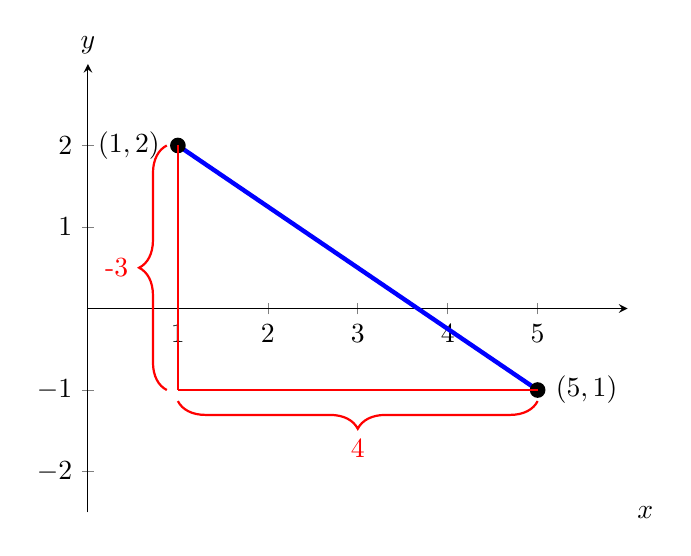
\begin{tikzpicture}
\begin{axis}[
    axis lines=middle,
    xlabel={$x$},
    ylabel={$y$},
    xlabel style={at={(rel axis cs:1,0)},anchor=west},
    ylabel style={at={(rel axis cs:0,1)},anchor=south},
    xmin=0, xmax=6,
    ymin=-2.5, ymax=3,
    xtick={0,1,...,5},
    ytick={-2,-1,...,2}
]

% Define the coordinates for the points
\coordinate (start) at (axis cs:1,2);
\coordinate (end) at (axis cs:5,-1);
\coordinate (origin) at (axis cs:1,-1);

% Draw the line
\addplot[blue, ultra thick, -] coordinates {(1,2) (5,-1)};

% Mark the points
\node[label={left:{$(1,2)$}},circle,fill,inner sep=2pt] at (start) {};
\node[label={right:{$(5,1)$}},circle,fill,inner sep=2pt] at (end) {};

% Draw the "rise"
\draw[red, thick] (start) -- (start|-origin) node [midway,left] {};

% Draw the "run"
\draw[red, thick] (start|-origin) -- (end) node [midway,below] {};

% Add curly brace for the "rise"
\draw [red, thick, decorate, decoration={brace, amplitude=10pt, raise=4pt}]
(origin) -- (start) node [midway, left, xshift=-5mm] {-3};

% Add curly brace for the "run"
\draw [red, thick, decorate, decoration={brace, amplitude=10pt, raise=4pt, mirror}]
(start|-origin) -- (end) node [midway, below, yshift=-5mm] {4};

\end{axis}
\end{tikzpicture}
\end{center}


Alternatively, since $\frac{3}{-4}$ represents the same number, the line can be drawn by starting at the point $(1, 2)$ and choosing a rise of 3 units followed by a run of $-4$ units. So from the point $(1, 2)$, we go up 3 units and to the left 4 units, thus reaching the point $(-3, 5)$, which is also on the same line. See figure below.
\begin{center}
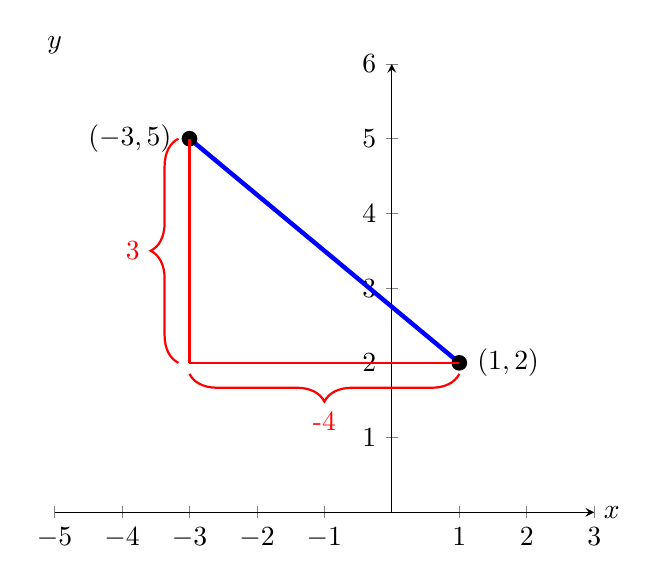
\begin{tikzpicture}
\begin{axis}[
    axis lines=middle,
    xlabel={$x$},
    ylabel={$y$},
    xlabel style={at={(rel axis cs:1,0)},anchor=west},
    ylabel style={at={(rel axis cs:0,1)},anchor=south},
    xmin=-5, xmax=3,
    ymin=0, ymax=6,
    xtick={-5,-4,...,3},
    ytick={0,1,...,6}
]

% Define the coordinates for the points
\coordinate (start) at (axis cs:-3,5);
\coordinate (end) at (axis cs:1,2);
\coordinate (origin) at (axis cs:-3,2);

% Draw the line
\addplot[blue, ultra thick, -] coordinates {(-3,5) (1,2)};

% Mark the points
\node[label={left:{$(-3,5)$}},circle,fill,inner sep=2pt] at (start) {};
\node[label={right:{$(1,2)$}},circle,fill,inner sep=2pt] at (end) {};

% Draw the "rise"
\draw[red, thick] (start) -- (start|-origin) node [midway,left] {};

% Draw the "run"
\draw[red, thick] (start|-origin) -- (end) node [midway,below] {};

% Add curly brace for the "rise"
\draw [red, thick, decorate, decoration={brace, amplitude=10pt, raise=4pt}]
(origin) -- (start) node [midway, left, xshift=-5mm] {3};

% Add curly brace for the "run"
\draw [red, thick, decorate, decoration={brace, amplitude=10pt, raise=4pt, mirror}]
(origin) -- (end) node [midway, below, yshift=-5mm] {-4};

\end{axis}
\end{tikzpicture}
\end{center}

\end{solution}
\begin{example}
Find the slope of the line $2x + 3y = 6$.	
\end{example}

\begin{solution}
In order to find the slope of this line, we will choose any two points on this line.
Again, the selection of $x$ and $y$ intercepts seems to be a good choice. The $x$-intercept is $(3, 0)$, and the $y$-intercept is $(0, 2)$. Therefore, the slope is
\[ m = \frac{2 - 0}{3 - 0} = \frac{-2}{3} .\]
The graph below shows the line and the $x$-intercepts and $y$-intercepts: 

\begin{center}
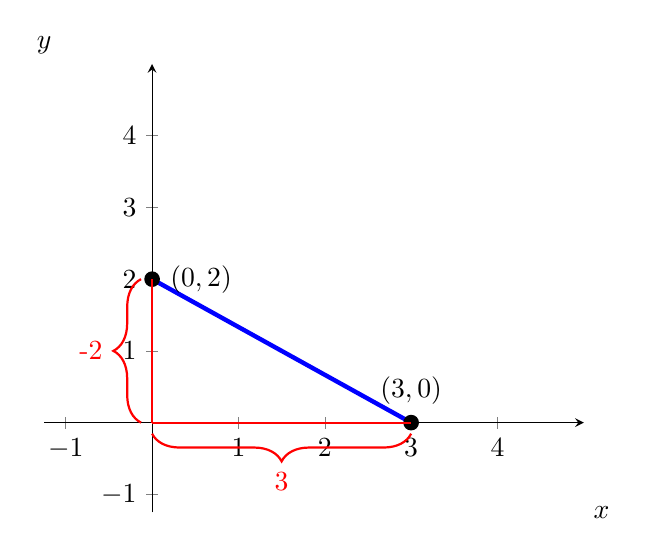
\begin{tikzpicture}
\begin{axis}[
    axis lines=middle,
    xlabel={$x$},
    ylabel={$y$},
    xlabel style={at={(rel axis cs:1,0)},anchor=west},
    ylabel style={at={(rel axis cs:0,1)},anchor=south},
    xmin=-1.25, xmax=5,
    ymin=-1.25, ymax=5,
    xtick={-1,0,...,4},
    ytick={-1,0,...,4}
]

% Define the coordinates for the points
\coordinate (start) at (axis cs:0,2);
\coordinate (end) at (axis cs:3,0);
\coordinate (origin) at (axis cs:0,0);

% Draw the line
\addplot[blue, ultra thick, -] coordinates {(0,2) (3,0)};

% Mark the points
\node[label={right:{$(0,2)$}},circle,fill,inner sep=2pt] at (start) {};
\node[label={above:{$(3,0)$}},circle,fill,inner sep=2pt] at (end) {};

% Draw the "rise"
\draw[red, thick] (start) -- (start|-end) node [midway,left] {};

% Draw the "run"
\draw[red, thick] (start|-end) -- (end) node [midway,below] {};

% Add curly brace for the "rise"
\draw [red, thick, decorate, decoration={brace, amplitude=10pt, raise=4pt}]
(origin) -- (start) node [midway, left, xshift=-5mm] {-2};

% Add curly brace for the "run"
\draw [red, thick, decorate, decoration={brace, amplitude=10pt, raise=4pt, mirror}]
(start|-origin) -- (end) node [midway, below, yshift=-5mm] {3};

\end{axis}
\end{tikzpicture}
\end{center}


\end{solution}


\begin{example}
Find the slope of the line $y = 3x + 2$.
\end{example}

\begin{solution} We again find two points on the line, say $(0, 2)$ and $(1, 5)$.
Therefore, the slope is
\[ m = \frac{5 - 2}{1 - 0} = \frac{3}{1} = 3.\]
\end{solution}
Look at the slopes and the $y$-intercepts of the following lines.
\begin{center}

\begin{tabular}{ccc}
Line & Slope & Y-Intercept \\
$y = 3x + 2$ & $3$ & $2$ \\
$y = -2x + 5$ & $-2$ & $5$ \\
$y = \frac{3}{2}x - 4$ & $\frac{3}{2}$ & $-4$
\end{tabular}
\end{center}

It is no coincidence that when an equation of the line is solved for $y$, the coefficient of the $x$ term represents the slope, and the constant term represents the $y$-intercept.
In other words, for the line $y = mx + b$, $m$ is the slope, and $b$ is the $y$-intercept.

\begin{example}
Determine the slope and $y$-intercept of the line $2x + 3y = 6$.
\end{example}

\begin{solution}
We solve for $y$:
\[2x + 3y = 6\]
\[3y = -2x + 6\]
\[y = -\frac{2}{3}x + 2\]
The slope is equal to the coefficient of the $x$ term, which is $-\frac{2}{3}$.
The $y$-intercept is equal to the constant term, which is $2$.
\end{solution}
